\section[Modèle relationnel]{Modèle relationnel}

%\subsection{Historique et définitions}

\begin{frame}
  \frametitle{Systèmes logiques : historique}
  \begin{itemize}
    \item Fichiers binaires et gérées par des programmes exécutables : modification de la structure des données très problématique
    \item SGBD hiérarchiques : Données organisées en arbre
    \item SGBD réseaux : Données organisées en graphe
    \item SGBD hiérarchiques et réseaux : dit navigationnels car on peut retrouver l'information à
      partir du chemin d'accès
    \item Pour chacun de ces systèmes, il existe des méthodes de traductions du MLD vers le MPD 
  \end{itemize}
\end{frame}

\begin{frame}
  \frametitle{Systèmes logiques : historique (2)}
  \begin{itemize}
    \item SGBD relationnels (SGBDR) : Information obtenue avec langage quasiment naturel (SQL pour
      Structured Query Langage)
    \item SGBD orientés objets : Il existe des \emph{framework} avec des \emph{mapping} objet-relationnel
      (\emph{ORM})
    \item Les bases de données NoSQL
      \begin{itemize}
        \item Relachement des propriétés ACID
        \item Permet la gestion d'un très grand nombre de données\\(\emph{Big Data})
      \end{itemize}
    \item Pour ce cours : modèle logique relationnel, abrégé:\\\og modèle relationnel \fg
  \end{itemize}
\end{frame}

\begin{frame}
  \frametitle{Modèle logique de données}
  \begin{itemize}
    \item Le modèle logique de données propose une modélisation plus concrète 
    \item Il est proche du modèle physique de données (qui sera implémenté)
    \item Il peut être traduit directement depuis le modèle conceptuel de données
  \end{itemize}
\end{frame}

\begin{frame}
  \frametitle{Tables, lignes et colonnes}
  \begin{itemize}
    \item Table : regroupe les données qui ont la même structure
    \item Colonne : décrit les champs en commun
    \item Ligne : contient les valeurs de ces champs pour un enregistrement
    \item Les lignes d'une table doivent être uniques
  \end{itemize}
  \begin{tabular}{c | c | c | c}
    numéro client & nom & prénom & adresse \\
    \hline \hline
    1 & Dupont & Michel & 127, rue\ldots \\
    2 & Durand & Jean & 314, boulevard\ldots \\
    3 & Dubois & Claire & 51, avenue\ldots \\
    4 & Dupuis & Marie & 2, impasse\ldots \\
    \ldots & \ldots & \ldots & \ldots
  \end{tabular}
  \begin{itemize}
    \item Exemple : table des renseignements clients
  \end{itemize}
\end{frame}

\begin{frame}
  \frametitle{Clés primaires}
  \begin{itemize}
    \item Clé primaire :
        \begin{itemize}
            \item Ensemble des colonnes permettant d'identifier une ligne
        \end{itemize}
    \item Une clé primaire ne peut avoir la valeur vide (NULL)
    \item La valeur de la clé primaire ne devrait pas changer au cours du temps
  \end{itemize}
\end{frame}

\begin{frame}
  \frametitle{Clés étrangères}
  \begin{itemize}
    \item Une colonne Colonne1 d'une table est clé étrangère ou référence la
        colonne Colonne2, si :
        \begin{itemize}
            \item Si elle ne contient que des valeurs prises par la colonne
                Colonne2 d'une autre table
            \item Colonne2 est sans doublons
        \end{itemize}
    \item Par convention, on souligne les clés primaires et on fait précéder les clés étrangères d'un dièse \#
      dans la description des colonnes d'une table :
    \item \texttt{clients(\underline{numéro client}, nom client, prénom, adresse client)}
    \item \texttt{commandes(\underline{numéro commande}, date de commande, \#numéro client (non vide))}
  \end{itemize}
\end{frame}

\begin{frame}
  \frametitle{Remarques}
  \begin{itemize}
    \item Une même table peut avoir plusieurs clés étrangères mais une seule clé primaire
    \item Une clé étrangère peut aussi être primaire (dans la même table)
    \item Une clé étrangère peut être composée (c'est le cas si la clé primaire référencée est composée)
    \item Chaque colonne qui compose une clé primaire ne peut pas recevoir la valeur vide (NULL)
%    \item Il est possible de préciser en SQL qu'une colonne doit pas recevoir la valeur vide (cf. suite du
%      cours)
%    \item Les SGBDR vérifient que chaque clé étrangère ne prend pas de valeurs en dehors de
%      celles déjà prises par la ou les colonne(s) qu'elle référence. Ce mécanisme qui agit lors de
%      l'insertion, de la suppression ou de la mise à jour de lignes dans les tables, garantit ce que l'on
%      appelle l'\emph{intégrité référentielle} des données.
  \end{itemize}
\end{frame}

\begin{frame}
  \frametitle{Schéma relationnel}
  \begin{itemize}
    \item Représentation des tables d'une base de données relationnelle par un schéma relationnel:
      \begin{itemize}
        \item Tables sont appelées \emph{relations}
        \item Liens entre les clés étrangères et leur clé primaire symbolisés par un connecteur
      \end{itemize}
    \end{itemize}
  \begin{center}
    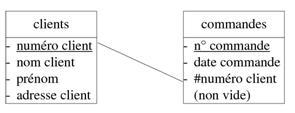
\includegraphics[width=0.7\linewidth]{schema_relationnel.jpg}
  \end{center}
\end{frame}

%\subsection{Traduction d'un modèle conceptuel en un modèle relationnel}

\begin{frame}
  \frametitle{Traduction d'un MCD en un MLDR}
  \begin{itemize}
    \item Pour traduire un MCD en un MLDR, il suffit d'appliquer cinq règles:
      \begin{enumerate}
        \item Traduction d'une entité
        \item Traduction d'une association binaire $1:n$
        \item Traduction d'une association binaire $n:m$
        \item Traduction d'une association binaire $1:1$
        \item Traduction d'une association non binaire
      \end{enumerate}
  \end{itemize}
\end{frame}

\begin{frame}
  \frametitle{Notations}
  \begin{itemize}
    \item Une association binaire est de type :
      \begin{itemize}
        \item $1 : 1$ (un à un) : si aucune des deux cardinalités maximales n'est $n$
        \item $1 : n$ (un à plusieurs) : si une des deux cardinalités maximales est $n$
        \item $n : m$ (plusieurs à plusieurs) : si les deux cardinalités maximales sont $n$
      \end{itemize}
    \item Un schéma relationnel ne peut faire la différence entre $0,n$ et $1,n$
    \item Par contre, il peut la faire entre $0,1$ et $1,1$
  \end{itemize}
\end{frame}

\begin{frame}
  \frametitle{Règle 1: Entité}
  \begin{itemize}
    \item Une entité devient une table:
      \begin{itemize}
        \item Les attributs deviennent les colonnes
        \item L'identifiant constitue la clé primaire de la table
      \end{itemize}
    \item Exemple :\\ L'entité article devient :\\\texttt{articles(\underline{numéro article}, désignation, prix unitaire de
      vente)}
  \end{itemize}
\end{frame}

\begin{frame}
  \frametitle{Règle 2 : Association binaire $1:n$ (1)}
  \begin{itemize}
    \item \texttt{fournisseurs(\underline{numero fournisseur}, nom contact, numero téléphone contact)}
    \item \texttt{livraisons(\underline{numero livraison}, date de livraison, nom livreur, \#numero fournisseur \text{(non
      vide)})}
  \end{itemize}
  \begin{center}
    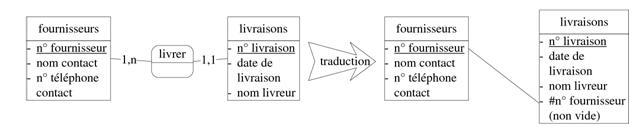
\includegraphics[width=0.9\linewidth]{traduction_1n.jpg}
  \end{center}
\end{frame}

\begin{frame}
  \frametitle{Règle 2 : Association binaire $1:n$ (2)}
  \begin{itemize}
    \item Une association binaire de type $1 : n$ disparaît:
      \begin{itemize}
        \item Au profit d'une clé étrangère dans la table côté $0,1$ ou $1,1$ qui référence la clé primaire de l'autre table
        \item Cette clé étrangère ne peut pas recevoir la valeur vide si la cardinalité est $1,1$
      \end{itemize}
    \item Il ne devrait pas y avoir d'attribut dans une association de type $1 : n$, s'il en reste, ils
      glissent vers la table côté 1.
  \end{itemize}
\end{frame}

\begin{frame}
  \frametitle{Règle 3 : Association binaire $n:m$ (1)}
  \begin{itemize}
    \item \texttt{lignes de commande(\underline{\#numero commande, \#numero article}, quantité commandée)}
  \end{itemize}
  \begin{center}
    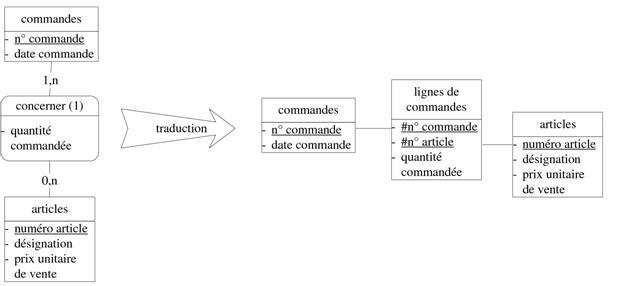
\includegraphics[width=0.9\linewidth]{traduction_nm.jpg}
  \end{center}
\end{frame}

\begin{frame}
  \frametitle{Règle 3 : Association binaire $n:m$ (2)}
  \begin{itemize}
    \item Une association binaire de type $n : m$ devient une table:
      \begin{itemize}
        \item La clé primaire est composée de deux clés étrangères (qui référencent les deux clés primaires
          des deux tables en association)
        \item Les attributs de l'association deviennent des colonnes de cette nouvelle table
      \end{itemize}
  \end{itemize}
\end{frame}

\begin{frame}
  \frametitle{Règle 4 : Association binaire $1:1$ (1)}
  \begin{itemize}
    \item \texttt{services(\underline{numero service}, nom service, \#numéro employé \text{(non vide, unique)})}
    \item \texttt{employés(\underline{numéro employé}, nom)}
  \end{itemize}
  \begin{center}
    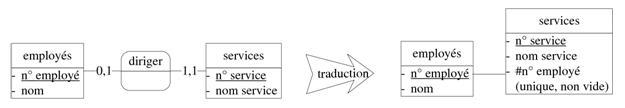
\includegraphics[width=0.9\linewidth]{traduction_11.jpg}
  \end{center}
\end{frame}

\begin{frame}
  \frametitle{Règle 4 : Association binaire $1:1$ (2)}
  \begin{itemize}
    \item Une association binaire de type $1 : 1$ est :
      \begin{itemize}
        \item Traduite comme une association binaire de type $1 : n$
        \item En plus, la clé étrangère se voit imposer une contrainte d'unicité
      \end{itemize}
    \item Si les associations fantômes ont été éliminées, il devrait y avoir au moins un côté de cardinalité
      $0,1$. C'est alors dans la table du côté opposé que doit aller la clé étrangère.
    \item Si les deux côtés sont de cardinalité $0,1$ alors la clé étrangère peut être placée indifféremment
      dans l'une des deux tables.
  \end{itemize}
\end{frame}

\begin{frame}
  \frametitle{Règle 5 : Association non binaire (1)}
  \begin{center}
    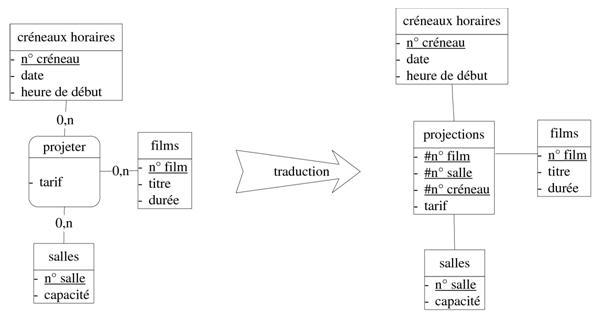
\includegraphics[width=0.9\linewidth]{traduction_non_binaire.jpg}
  \end{center}
\end{frame}

\begin{frame}
  \frametitle{Règle 5 : Association non binaire (2)}
  \begin{itemize}
    \item Une association non binaire est traduite par une table supplémentaire :
      \begin{itemize}
        \item La clé primaire est composée d'autant de clés étrangères que d'entités en association
        \item Les attributs de l'association deviennent des colonnes de cette nouvelle table
      \end{itemize}
  \end{itemize}
\end{frame}

%\subsection{Compléments}

\begin{frame}
  \frametitle{Optimisation (1)}
  \begin{itemize}
    \item L'optimisation des performances en temps de calcul se fait toujours au détriment de l'espace mémoire
      consommé
    \item Dans le pire des cas, réduire les temps de réponse consiste à dé-normaliser volontairement le
      système d'information, avec tous les risques d'incohérence et les problèmes de gestion que cela
      comporte
    \item Le conseil le plus précieux, en matière d'optimisation, est de ne jamais optimiser \emph{a priori},
      mais toujours \emph{a posteriori} :
    \item[$\ra$] C'est-à-dire en réponse à une lenteur que le SGBDR n'est pas capable de résoudre tout seul
    \item Il convient de mesurer le gain de toute optimisation manuelle en effectuant des tests
      (chronométrages avant/après) sur un volume de données significatif et de préférence en exploitation
  \end{itemize}
\end{frame}

\begin{frame}
  \frametitle{Optimisation (2)}
  \begin{itemize}
    \item Pour les bases de données relationnelles, l'optimisation peut passer par :
      \begin{itemize}
        \item L'ajout d'index aux tables (au minimum sur les colonnes clés primaires et clés étrangères):
          \begin{itemize}
            \item Ces index consomment de l'espace mémoire supplémentaire
            \item La base de données reste normalisée
          \end{itemize}
        \item L'ajout de colonnes calculées ou de certaines redondances :
          \begin{itemize}
            \item Permet d'éviter des jointures coûteuses
            \item La base est dé-normalisée
            \item Il faut alors veiller à ce que la cohérence entre les colonnes soit respectée (déclencheurs
              ou code client)
          \end{itemize}
        \item La suppression des contraintes :
          \begin{itemize}
            \item D'unicité, de clé étrangère, etc.
            \item L'intégrité des données doit être assurée par le code client
          \end{itemize}
      \end{itemize}
  \end{itemize}
\end{frame}

\begin{frame}
  \frametitle{Optimisation : Exemple}
  \begin{itemize}
    \item La table commandes peut être supprimée et la date de commande est alors ajoutée à la table lignes de
      commandes
  \end{itemize}
  \begin{center}
    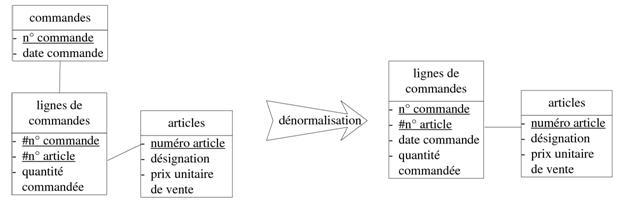
\includegraphics[width=0.9\linewidth]{optimisation.jpg}
  \end{center}
  \begin{itemize}
    \item On renonce donc à la troisième forme normale :
      \begin{itemize}
        \item La date de commande est répétée autant de fois qu'il y a de lignes dans la commande
        \item Mais on évite une jointure coûteuse en temps de calcul lors des requêtes SQL
      \end{itemize}
  \end{itemize}
\end{frame}

\begin{frame}
  \frametitle{Héritage (1)}
  \begin{itemize}
    \item Factorisation des attributs communs à plusieurs entités au sein d'une entité mère
  \end{itemize}
  \begin{center}
    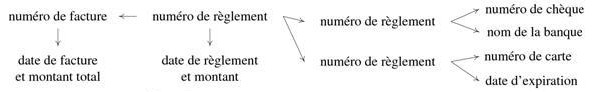
\includegraphics[width=0.9\linewidth]{heritage_1.jpg}
  \end{center}
  \begin{itemize}
    \item Exemple :
      \begin{itemize}
        \item Factures de paiement par chèque ou par carte
        \item On souhaite connaître pour chaque règlement la \emph{date} et le \emph{montant}
      \end{itemize}
  \end{itemize}
\end{frame}

\begin{frame}
  \frametitle{Héritage (2)}
  \begin{center}
    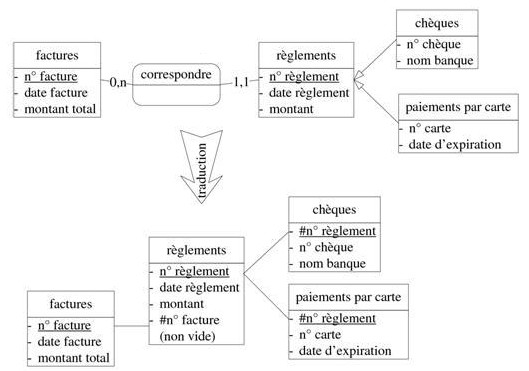
\includegraphics[width=0.7\linewidth]{heritage_2.jpg}
  \end{center}
  \begin{itemize}
    \item[$\ra$] Une entité générique règlements et deux entités spécialisées chèques et paiements par carte
    \item Lien d'héritage représenté par une flèche creuse\\ 
       (ce lien remplace une association de type $1 : 1$)
  \end{itemize}
\end{frame}

\begin{frame}
  \frametitle{Héritage (3)}
  \begin{itemize}
    \item Les deux sous-entités de l'entité règlements ont des attributs propres mais pas d'identifiant
      propre
    \item Il ne faut pas voir d'héritage à chaque fois que l'on peut dire « est un » :\\
      il faut en plus que l'entité mère ne possède que les attributs communs de ses entités filles
    \item La traduction des sous-entités au niveau logique relationnel fait intervenir une clé primaire
      identique à celle de l'entité mère, mais dans les sous-entités la clé primaire est aussi étrangère
  \end{itemize}
\end{frame}

\begin{frame}
  \frametitle{Héritage et informations complémentaires}
  \begin{itemize}
    \item L'héritage est également utile pour stocker des informations complémentaires
  \end{itemize}
  \begin{center}
    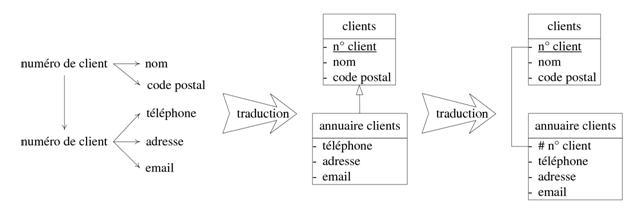
\includegraphics[width=0.9\linewidth]{heritage_informations_complementaires.jpg}
  \end{center}
  \begin{itemize}
    \item Exemple :
      \begin{itemize}
        \item Table clients avec numéro, nom et code postal
        \item Ajout de trois colonnes mais il y a déjà des valeurs saisies
        \item[$\ra$] Une nouvelle table permet de gagner de la place
      \end{itemize}
  \end{itemize}
\end{frame}

\begin{framentitle}{Héritage et contraintes (1)}
    \begin{itemize}
       \item Il est possible de préciser sur le modèle conceptuel des
            contraintes sur l'héritage :
            \begin{itemize}
                \item Exclusivité ($X$): équivaut à un «~OU exclusif~». On est l'une,
                    l'autre ou aucune, mais pas les deux à la fois.
                \item Totalité ($T$) : équivaut à un «~OU~». On est l'une,
                    l'autre, les deux, mais pas aucune des deux.
                \item Partition ($XT$) : totalité + exclusivité. On est l'une ou
                    l'autre (et donc ni les deux, ni aucune des deux).
                \item Vide : on est l'une, l'autre, les deux ou aucune des deux.
            \end{itemize}
    \end{itemize}
\end{framentitle}

\begin{framentitle}{Héritage et contraintes (2)}
    \begin{center}
    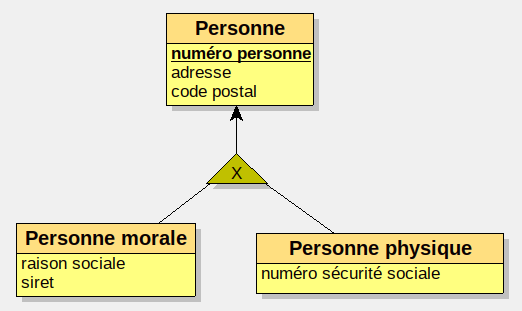
\includegraphics[width=.8\textwidth]{heritage_x.png}
    \end{center}
    \begin{itemize}
        \item Exclusivité ($X$): équivaut à un «~OU exclusif~».\\On est l'une,
            l'autre ou aucune, mais pas les deux à la fois.
    \end{itemize}
\end{framentitle}

\begin{framentitle}{Héritage et contraintes (3)}
    \begin{center}
    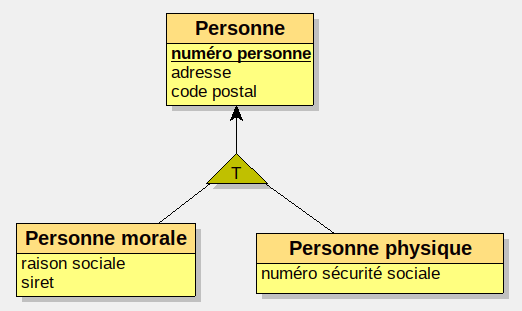
\includegraphics[width=.8\textwidth]{heritage_t.png}
    \end{center}
    \begin{itemize}
        \item Totalité ($T$) : équivaut à un «~OU~».\\On est l'une, l'autre, les
            deux, mais pas aucune des deux.
    \end{itemize}
\end{framentitle}

\begin{framentitle}{Héritage et contraintes (4)}
    \begin{center}
    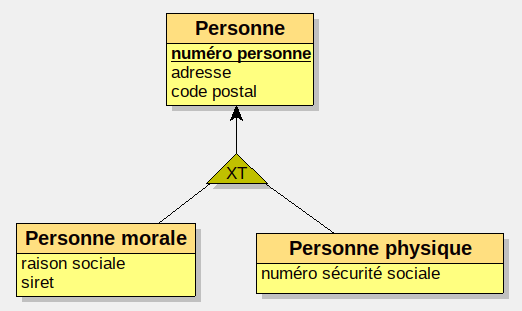
\includegraphics[width=.8\textwidth]{heritage_xt.png}
    \end{center}
    \begin{itemize}
        \item Partition ($XT$) : totalité + exclusivité.\\On est l'une ou l'autre
            (et donc ni les deux, ni aucune des deux).
    \end{itemize}
\end{framentitle}

\begin{framentitle}{Héritage et contraintes (5)}
    \begin{center}
    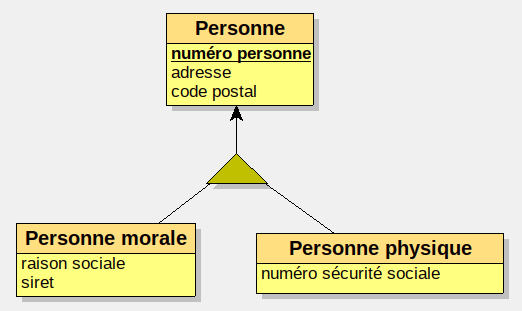
\includegraphics[width=.8\textwidth]{heritage_vide.png}
    \end{center}
    \begin{itemize}
        \item Vide :\\On est l'une, l'autre, les deux ou aucune des deux.
    \end{itemize}
\end{framentitle}

